\documentclass[letterpaper]{article}
\usepackage{csc-poster}
\usepackage{hyperref}

\begin{document}

\cschead{\emph{To Mock a Mockingbird} Reading Group}{}

%\cscsubtitle{Let's go on an amazing adventure in combinatory logic!}
\cscsubtitle{These birds must pay for their hubris!}

\emph{To Mock a Mockingbird and Other Logic Puzzles: Including an Amazing Adventure in Combinatory Logic} is a book by the mathematician and logician Raymond Smullyan. It contains many nontrivial recreational puzzles of the sort for which Smullyan is well known. It is also a gentle and humorous introduction to combinatory logic and the associated metamathematics, built on an elaborate ornithological metaphor. 

\vspace{0.75in}
\begin{tabular}{rl}
    \csctimefont Book: & \url{https://bit.ly/3GXeiuf}  \\
    & \\
    \csctimefont Discord Server: & \url{https://discord.gg/95Utp8byPW}
\end{tabular}

\vspace{0.5in}
\begin{center}
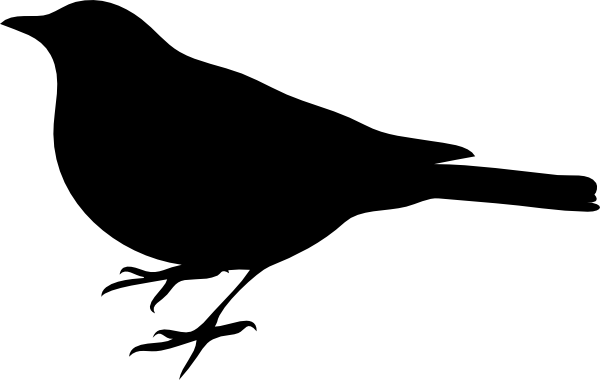
\includegraphics[scale = 0.75]{mockingbird_logo.png}
\end{center}

\cscsubtitle{Next Session Begins In May}
\vspace{-15pt}
\cscsubtitle{Latecomers Accepted}
\vspace{-15pt}
\centering \cscsubtitle{\small All the cool kids are doing it; don't you wanna be \emph{cool}?}

\end{document}